\documentclass[runningheads]{llncs}
\usepackage{graphicx}
\usepackage{diagbox}
\usepackage{amsmath}
\usepackage{amssymb}
\usepackage[spanish]{babel}
\usepackage{hyperref}
%
\begin{document}
	\hyphenation{}
	
	\title{Proyecto Final de Sistemas de Recuperaci\'on de Informaci\'on}
	
	\author{Rocio Ortiz Gancedo \and Carlos Toledo Silva}
	
	\institute{Universidad de La Habana, Cuba}
	
	\titlerunning{Proyecto Final de Sistemas de Recuperaci\'on de Informaci\'on}
	
	\maketitle
	
	\begin{abstract}
		Desde el surgimiento del almacenamiento de informaci\'on, poder acceder a esta de forma c\'omoda y eficiente cuando se necesite, ha sido de gran importancia. Con la aparici\'on de las computadoras esto se ha podido automatizar mediante programas, conocidos como Sistemas de Recuperaci\'on de Informaci\'on. El proyecto que se presenta constituye un Sistema de Recuperaci\'on de Informaci\'on para un conjunto de documentos utilizando el modelo vectorial. En este art\'iculo se describe todo el proceso de dise\~{n}o, implementaci\'on y an\'alisis de los resultados del sistema.
	\end{abstract}

	\section{Introducci\'on}
La b\'usqueda y recuperaci\'on de informaci\'on es la ciencia que estudia la manera de hallar los datos en documentos electr\'onicos y cualquier tipo de colecci\'on documental digital. 

Inicialmente el manejo a grandes vol\'umenes de informaci\'on ocurr\'ia con las bibliotecas. Para acceder c\'omodamente a los libros y art\'iculos se manten\'ian indexados usando cat\'alogos. Desde 1891 se comienzan a utilizar equipos para automatizar la b\'usqueda en los mismos. 

En los a\~{n}os 40 se emplea por primera vez el t\'ermino Recuperaci\'on de Informaci\'on y ya en los 50 comienzan a usarse computadoras para este fin.
 
El proceso de recuperaci\'on de informaci\'on comienza cuando un usuario hace una consulta al sistema. Dentro de los modelos de Sistemas de Recuperaci\'on de Informaci\'on encontramos el modelo vectorial que fue el que se desarroll\'o en este proyecto que a continuaci\'on se presenta.

El objetivo de este proyecto es brindar un Sistema de Recuperaci\'on de Informaci\'on para una colecci\'on de datos dada y presentar un informe donde se explique bien el mismo.

El resto del documento est\'a dividido en seis secciones principales. En la secci\'on 2 se incluye el dise\~{n}o del sistema, donde se explica brevemente este modelo, las razones para la selecci\'on del mismo y algunas ideas interesantes que se tuvieron en cuenta en la concepci\'on del sistema. La secci\'on 3 aborda la implementaci\'on del sistema, explicando c\'omo se procesaron y se representaron los documentos y consultas. Se incluye tambi\'en la explicaci\'on de como se hace el an\'alisis de similitud entre las consultas y los documentos. Adem\'as se explica c\'omo se realiz\'o la retroalimentaci\'on y muestra el funcionamiento de la interfaz gr\'afica. La secci\'on 4 eval\'ua el sistema que se implement\'o, muestra  las medidas usadas para esto y los resultados obtenidos. Estas evaluaciones se realizaron utilizando la colecciones \textbf{Cranfield} y \textbf{Medline}. La secci\'on 5 realiza un an\'alisis cr\'itico de las ventajas y desventajas de la aplicaci\'on. Por \'ultimo en la secci\'on 6 y 7 se encuentran las conclusiones y recomendaciones respectivamente. 

	\section{Dise\~{n}o del sistema}
	
	\subsection{Recordatorio de las caracter\'isticas del modelo vectorial}
	
	En el modelo vectorial, el peso $w_{i,j}$ asociado al par $(t_i,d_j)$ (siendo $t_i$ el t\'ermino $i$ y $d_j$ el documento $j$) es positivo y no binario. A su vez, los t\'erminos en la consulta est\'an ponderados. Sea $w_{i,q}$ el peso asociado al par $(t_i,q)$ (siendo $q$ una consulta), donde $w_{i,q}\geq 0$. Entonces, el vector consulta $q$ se define como $\overrightarrow{q}=(w_{1q},w_{2q},...,w_{nq})$ donde $n$ es la cantidad total de t\'erminos indexados en el sistema. El vector de un documento $d_j$ se representa por $\overrightarrow{d_j}=(w_{1j},w_{2j},...,w_{nj})$.
	
	La correlaci\'on se calcula utilizando el coseno del \'angulo comprendido entre los vectores documentos $dj$ y la consulta $q$.
	
	\begin{equation}
		sim(d_j,q)=\frac{\overrightarrow{d_j}\cdot\overrightarrow{q}}{|\overrightarrow{d_j}|\cdot|\overrightarrow{q}|}
	\end{equation}

	\begin{equation}	
		sim(d_j,q)=\frac{\sum_{i=1}^{n}w_{i,j}\cdot w_{i,q}}{\sqrt{\sum_{i=1}^{n}w_{i,j}^2}\cdot\sqrt{\sum_{i=1}^{n}w_{i,q}^2}}
	\end{equation}  

	Sea $freq_{i,j}$ la frecuencia del t\'ermino $t_i$ en el documento $d_j$. Entonces, la frecuencia normalizada $tf_{i,j}$ del t\'ermino $t_i$ en el documento $d_j$ est\'a dada por:
	
	\begin{equation}
		tf_{i,j}=\frac{freq_{i,j}}{max_lfreq_{l,j}}
	\end{equation}

	donde el m\'aximo se calcula sobre todos los t\'erminos del documento $d_j$. Si el t\'ermino $t_i$ no aparece en el documento $d_j$ entonces $tf_{i,j}=0$.
	
	Sea $N$ la cantidad total de documentos en el sistema y $n_i$ la cantidad de documentos en los que aparece el t\'ermino $t_i$. La frecuencia de ocurrencia de un t\'ermino $t_i$ dentro de todos los documentos de la colecci\'on $idf_i$ est\'a dada por:
	
	\begin{equation}
		idf_i=\log \frac{N}{n_i}
	\end{equation}

	El peso del t\'ermino $t_i$ en el documento $d_j$ est\'a dado por:
	
	\begin{equation}
		w_{i,j}=tf_{i,j}\cdot idf_i
	\end{equation}

	El c\'alculo de los pesos en la consulta $q$ se hace de la siguiente forma:
	
	\begin{equation}
		w_{i,q}=\left\{\begin{array}{c}
			0,~si~freq_{i,q}=0\\
			\left(a+(1-a)\frac{freq_{i,q}}{max_lfreq_{l,q}}\right)\cdot\log \frac{N}{n_i},~en~otro~caso
		\end{array}\right. 
	\end{equation}

	donde $freq_{i,q}$ es la frecuencia del t\'ermino $t_i$ en el texto de la consulta $q$. El t\'ermino $a$ es de suavizado y permite amortiguar la contribuci\'on de la frecuencia del t\'ermino, toma un valor entre 0 y 1. Los valores m\'as usados son 0.4 y 0.5. 
	
	\subsection{\textquestiondown Por qu\'e seleccionamos el modelo vectorial?}
	
	Se seleccion\'o el modelo vectorial primeramente por la amplia cantidad de elementos impartidos durante el curso sobre este modelo. Adem\'as este presenta las siguientes ventajas:
	
	\begin{itemize}
		\item El esquema de ponderaci\'on $tf-idf$ para los documentos mejora el rendimiento de la recuperaci\'on.
		\item La estrategia de coincidencia parcial permite la recuperaci\'on de documentos que se aproximen a los requerimientos de la consulta.
		\item La f\'ormula del coseno ordena los documentos de acuerdo al grado de similitud.
	\end{itemize}

	Adem\'as de estas ventajas tambi\'en cabe destacar la muy buena posibilidad de retroalimentaci\'on que admite este modelo.
	
	\subsection{Ideas interesantes}
	
	\subsubsection{Usar diccionarios para representar a los vectores y las consultas}
	Una idea interesante que utilizamos para representar lo que son los vectores en la teor\'ia, como los vectores de los t\'erminos y de pesos tanto de los documentos como de las consultas, en lugar de como vectores, los implementamos como diccionarios, tal que la clave es el t\'ermino $i$ (preprocesado) y el valor correspondiente a dicha clave seg\'un cual sea el diccionario, ser\'ia la frecuencia o el peso del t\'ermino en un documento o consulta en espec\'ifico. 
	
	Esto lo hacemos debido a la gran cantidad de t\'erminos que pudieran haber en una colecci\'on grande de documentos y representar cada documento mediante un vector de longitud igual a la cantidad total de t\'erminos distintos ser\'ia altamente costoso en memoria y en tiempo de ejecuci\'on. Adem\'as de la gran probabilidad de que la matriz conformada por los vectores de frecuencia de los t\'erminos y en consecuencia la matriz formada por los vectores de pesos de los t\'erminos en los documentos sean muy esparcidas, pues lo m\'as probable, si se tiene una colecci\'on grande de documentos, es que un t\'ermino $t_i$, si es relevante, aparezca en una cantidad muy inferior de documentos con respecto al total de los mismos.
	
	Adem\'as esto lo podemos hacer debido a que un t\'ermino que no aparezca en un documento, dado que su frecuencia es cero y por como se calculan los pesos y la similitud entre un documento y una consulta, no afecta para nada el c\'alculo de estos par\'ametros. Veamos esto r\'apidamente:
	
	Por (2) tenemos en el numerador una sumatoria donde el t\'ermino $i$ de la sumatoria es 0 si $w_{i,j}=0 \lor w_{i,q}=0$. Por (5) tenemos que $w_{i,j}=0$ si $tf_{i,j}=0 \lor idf_i=0$. Luego por (3) tenemos que $tf_{i,j}=0$ si $freq_{i,j}=0$, o sea si el t\'ermino $t_i$ no aparece en el documento $d_j$
	
	Para la consulta, por (6) tenemos que si la $freq_{i,q}=0$ entonces $w_{i,q}=0$.
	
	Por tanto si el t\'ermino $t_i$ no aparece en el documento o no aparece en la consulta, entonces $t_i$ no influye en la sumatoria del numerador.
	
	Pasemos entonces a analizar el denominador. En este tenemos dos sumatorias: una que itera por los cuadrados de los pesos del vector del documento y otra que itera por los cuadrados de los pesos del vector de la consulta. Es evidente que si el peso de $t_i$ en $d_j$ es 0 entonces este no influye en la sumatoria. Lo mismo ocurre si un t\'ermino no aparece en la consulta $q$.
	
	Por tanto llegamos a la conclusi\'on que para calcular la similitud entre una consulta y un documento solo necesitamos los t\'erminos que aparecen en el documento o en la consulta.
	
	 \subsubsection{Guardar volúmenes de informaci\'on en .json, sobre todo aquellas que se utilizan mucho} De esta forma se devid\'ia la ejecuci\'on en partes, en vez de hacerlo todo de una vez lo cual se demorar\'ia un tiempo considerable y adem\'as cada vez que se quisiera correr el sistema se estar\'ian haciendo los mismos c\'alculos. Algunos objetos guardados en .json son la representaci\'on de los vectores de los documentos y las consultas y un diccionario que contiene a cada t\'ermino con su respectivo $idf_i$. Los adjuntados en este trabajo son los referentes a los de la colecci\'on Medline.
	
	\subsubsection{Utilizar un heap para llevar el ranking de similitud de una consulta} Utilizando esta estructura llevamos un orden parcial de las similitudes de una consulta con los documentos en el sistema.
		
	\section{Implementaci\'on del sistema}
	
	\subsection{Preprocesamiento de los documentos}
	
	Las funciones para el preprocesamiento de los documentos de una colecci\'on las podemos encontrar en ``collection\_preprocess.py''. Primero tenemos la funci\'on \verb|collection_preprocessing| la cual, a partir de la colecci\'on de documentos, devuelve un diccionario tal que las llaves son los t\'erminos que aparecen en los documentos y el valor asociado a cada t\'ermino es el conjunto de los documentos en los que aparece dicho t\'ermino. Los t\'erminos a su vez son sometidos a un preprocesamiento y para esto utilizamos la librer\'ia \verb|nltk|.
	
	El proceso de tokenizaci\'on se hace mediante la funci\'on \verb|word_tokenize| la cual a partir de un texto(por defecto en ingl\'es) devuelve los diferentes tokens de dicho texto. Luego los tokens son clasificados sint\'acticamente y etiquetados con dicha clasificaci\'on mediante el m\'etodo \verb|pos_tag|. Esto se hace pues para el proceso de ``\textit{lemmatizing}''(llevar las palabras a su ra\'iz gramatical) que es el proceso que viene a continuaci\'on, tener los tokens clasificados mejora el rendimiento de este proceso. Despu\'es de realizado
	el proceso de \textit{lemmatizing}, se chequea si los t\'erminos obtenidos son ``\textit{stopwords}''(palabras que no proveen informaci\'on \'util). Si un t\'ermino $i$ no es una \textit{stopword}, si no est\'a en el diccionario, se a\~{n}ade como llave y se crea un conjunto con el documento actual. Si ya est\'a el t\'ermino en el diccionario entonces se a\~{n}ade al conjunto correspondiente al t\'ermino el documento actual. Como es un conjunto si el documento ya est\'a en el conjunto, este no se agregar\'a.
	
	Debido a que se analizan todos los documentos de una colecci\'on y de cada uno de estos se analizan todos sus t\'erminos, asumiendo que todas las operaciones que se realizan sobre un token se hacen en $O(1)$, llegamos a la conclusi\'on que una llamada a esta funci\'on tiene una complejidad temporal $O(n\cdot m)$; siendo $n$ la cantidad total de documentos y $m$ la cantidad de tokens del documento que mayor cantidad de tokens tiene.
	
	La otra funci\'on que aparece en este archivo es \verb|terms_freq_doc|, la cual devuelve de forma perezosa un diccionario para cada documento de la colecci\'on y un valor entero. El diccionario tiene como llaves los t\'erminos que aparecen en dicho documento y el valor asociado a cada t\'ermino es la frecuencia del t\'ermino en el documento. El n\'umero entero que se devuelve junto con el diccionario es la frecuencia del t\'ermino de mayor frecuencia en el documento. Cada vez que se detecte un documento nuevo, se crea un diccionario y un entero inicializado con 0. El procesamiento de los t\'erminos se hace de forma similar que en el m\'etodo anterior. Por cada t\'ermino $i$ en el documento $j$ se verifica si ya este fue agregado al diccionario. En caso afirmativo se incrementa en 1 su valor asociado y en caso contrario se agrega el t\'ermino al diccionario, asoci\'andole 1 como valor, pues es la primera vez que se detecta. Despu\'es de esto se comprueba si dado este aumento la frecuencia del t\'ermino aument\'o, de tal forma que se hizo mayor que la m\'axima frecuencia detectada hasta el momento para el documento. De ocurrir lo antes planteado se actualiza entonces la m\'axima frecuencia detectada (la variable \verb|max_freq|). Cada vez que se termine de analizar un documento se devuelve el diccionario y el entero antes mencionado.
	
	Como se explic\'o una ejecuci\'on completa de este m\'etodo analiza cada uno de los documentos y sus tokens. Adem\'as realiza una gran cantidad de operaciones similares a las que se hacen en la funci\'on anterior y las que tiene diferente con respecto al otro tienen una complejidad temporal despreciable (son $O(1)$). Por tanto llegamos a la conclusi\'on que una ejecuci\'on completa de este m\'etodo es $O(n\cdot m)$, siendo $n$ y $m$ los mismos valores mencionados anteriormente.
	
	\subsection{Representaci\'on de los documentos}
	
	El c\'odigo relacionado a este apartado lo podemos encontrar en\\ ``docs\_representation.py''. Primero veamos como hallar los valores $idf_i$ para los diferentes t\'erminos. Estos valores se calculan utilizando la funci\'on \verb|calculate_idfs| la cual recibe un diccionario que tiene como llaves a los diferentes t\'erminos y el objeto asociado a un t\'ermino $t_i$ es el conjunto de documentos en los que el t\'ermino $t_i$ aparece; adem\'as de un valor entero que indica la cantidad de documentos que hay en el sistema. M\'as concretamente este m\'etodo recibe la salida del m\'etodo \verb|collection_preprocessing| u otro que de una salida similar. Est\'e m\'etodo devuelve un diccionario que tiene como llaves a cada uno de los t\'erminos, y el valor asociado a cada t\'ermino $t_i$ es su respectivo valor $idf_i$. Lo que se hace dentro del m\'etodo es lo siguiente: 

	\begin{itemize}
		\item Crear el diccionario \verb|idfs|.
		\item Por cada t\'ermino en el diccionario de entrada:
		\begin{itemize}
			\item Calcular su $idf_i$ correspondiente y guardar la pareja $t_i$ y $idf_i$ en el diccionario \verb|idfs| como llave y valor respectivamente.
		\end{itemize}
		\item  Retornar el diccionario \verb|idfs|.
	\end{itemize}
	 
	Es sencillo notar que la complejidad temporal de esta funci\'on es $O(k)$, siendo $k$ el n\'umero total de t\'erminos.
	
	Veamos ahora como calcular los valores $tf_{i,j}$ para cada t\'ermino en un documento. La funci\'on utilizada para esto es \verb|calculate_tfijs| que recibe un objeto iterable, tal que cada elemento del objeto iterable es una tupla $<$diccionario, entero$>$. El diccionario tiene como llaves los t\'erminos que aparecen en un documento $d_j$ y el entero indica la frecuencia del t\'ermino de mayor frecuencia en el documento $d_j$. Este m\'etodo retorna de forma perezosa un diccionario por cada documento $d_j$ que contiene como llave los t\'erminos de dicho documento y para cada t\'ermino su valor asociado es el valor $tf_{i,j}$ correspondiente. La forma de hacer esto es:
	
	\begin{itemize}
		\item Por cada elemento del objeto iterable:
		\begin{itemize}
			\item Crear el diccionario \verb|tfj|
			\item Por cada t\'ermino en el diccionario obtenido del objeto iterable:
			\begin{itemize}
				\item Calcular el $tf_{i,j}$ correspondiente y guardar dicha pareja en el diccionario \verb|tfj|
			\end{itemize}
			\item Retornar \verb|tfj| 
		\end{itemize}
	\end{itemize}
	
	La idea de hacerlo de forma perezosa es no tener en memoria grandes vol\'umenes de informaci\'on que no son necesarios en todo momento. Ya que se analizan los $n$ documentos de la colecci\'on y en cada una la cantidad de t\'erminos es $O(m)$, una ejecuci\'on completa de este m\'etodo es $O(n\cdot m)$.
	
	Como ya vimos como calcular $idf$ y $tf$ a continuaci\'on se explicar\'a como calcular entonces los ``vectores'' de pesos para cada uno de los documentos.  Esto se hace mediante la funci\'on \verb|calculate_weights|. Esta funci\'on recibe, como primer argumento, el mismo argumento que recibe la funci\'on \verb|calculate_tfijs| descrita anteriormente, y como segundo argumento, un diccionario que contiene los t\'erminos y sus respectivos $idf_i$. Su funcionamiento es el siguiente:
	
	\begin{itemize}
		\item Crear una lista \verb|vec_docs|, que ser\'a en la que se ir\'an guardando los ``vectores'' de pesos
		\item Por cada elemento que devuelve el llamado a la f\'uncion \verb|calculate_tfijs| (recordemos que cada elemento devuelto es un diccionario con los t\'erminos de un documento $d_j$ y sus respectivos $tf_{i,j}$):
		\begin{itemize}
			\item Crear el diccionario \verb|vec_weights|
			\item Por cada uno de los t\'erminos del diccionario devuelto:
			\begin{itemize}
				\item Calcular su peso y guardar la pareja t\'ermino y peso en el diccionario \verb|vec_weights|
			\end{itemize}
			\item A\~{n}adir \verb|vec_weights| a la lista \verb|vec_docs|
		\end{itemize}
		\item Retornar \verb|vec_docs|.
	\end{itemize}
	
	En este m\'etodo se hace un llamado a \verb|calculate_tfijs| la cual sabemos que tiene complejidad temporal $O(n\cdot m)$ y se itera por los $n$ elementos que esta devuelve y por cada uno se recorre una cantidad $O(m)$ de t\'erminos. Por tanto la complejidad temporal de esta funci\'on es $O(n\cdot m)$.
	
	Ejecutando este archivo se calculan y se guardan en archivos .json los vectores de pesos de los documentos y los valores $idf_i$ de los t\'erminos. Para especificar la colecci\'on deseada se debe indicar la direcci\'on en la variable \verb|collection| de la l\'inea 36.
	
	\subsection{Preprocesamiento de las consultas}
	
	El preprocesamiento de las consultas se hace de una forma parecida al preprocesamiento de los documentos. El c\'odigo referente a este apartado se encuentra en el archivo ``queries\_preprocess''.
	
	La primera funci\'on ``query\_preprocessing'' se utiliza para preprocesar una sola consulta. Recibe el texto de una consulta y el diccionario \verb|idfs| que contiene a los t\'erminos con sus respectivos valores de $idf$. Una consulta se procesa de la misma manera que un documento, lo que con un paso extra: luego de que un token haya sido completamente procesado se comprueba si pertenece al diccionario \verb|idfs|, pues solo interesan las palabras que pertenezcan al menos a un documento de la colecci\'on. Este m\'etodo devuelve un diccionario con los t\'erminos de la consulta y sus respectivas frecuencias, adem\'as de un entero que indica la frecuencia m\'axima de un t\'ermino en la consulta. Su complejidad temporal es $O(m)$, siendo $m$ la cantidad de palabras de la consulta. 
	
	El siguiente m\'etodo ``queries\_preprocessing'' se utiliza para el preprocesamiento de las consultas de la colecci\'on. Devuelve de forma perezosa el diccionario y el entero explicados anteriormente para cada una de las consultas en la colecci\'on. Su complejidad temporal es $O(n\cdot m)$ siendo $n$ el n\'umero de consultas y $m$ la cantidad de tokens de la consulta con mayor cantidad de tokens.
	
	\subsection{Representaci\'on de las consultas}
	
	El c\'odigo para calcular los pesos de las consultas se encuentra en el archivo ``queries\_representation.py''. En este se haya la funci\'on ``calculate\_weigths\_queries'' que recibe un valor para $a$, el diccionario \verb|idfs| y un objeto iterable, donde cada elemento de este es una tupla $<$diccionario,entero$>$, tal que el diccionario contiene los t\'erminos de una consulta y su frecuencia en la misma y el entero indica la frecuancia m\'axima de un t\'ermino en la consulta. Esta devuelve una lista con la representaci\'on en pesos de las consultas pasadas en el objeto iterable. La definici\'on de la funci\'on es muy similar a la utilizada para calcular los pesos de los documentos; el \'unico cambio es el de utilizar adem\'as la constante $a$ de suavizado para el c\'alculo de los pesos de una consulta. La complejidad temporal es $O(n\cdot m)$.
	
	Ejecutando este archivo se guarda en un archivo .json los pesos de las consultas de la colecci\'on. Para especificar la colecci\'on deseada se debe indicar la direcci\'on en la variable \verb|collection| de la l\'inea 25.
	
	\subsection{Similitud entre documentos y consultas}
	
	El c\'odigo relacionado  a este apartado se encuentra en el archivo\\ ``similarity.py''. La primera funci\'on que se aprecia es \verb|sim_doc_query|. Esta recibe los ``vectores'' de pesos de un documento y una consulta (que recordemos son diccionarios) y devuelve un n\'umero que representa la similitud entre el documento y la consulta. La forma de proceder es la siguiente:
	
	\begin{itemize}
		\item Si el documento o la consulta no tiene t\'erminos entonces la similitud es 0.
		
		\item Se calcula $\overrightarrow{d_j}\cdot\overrightarrow{q}$ utilizando solo los t\'erminos que tienen en com\'un ambos
		
		\item Se calcula $|\overrightarrow{d_j}|$ con todos los t\'erminos de $d_j$
		
		\item Se calcula $|\overrightarrow{q}|$ con todos los t\'erminos de $q$
		
		\item Se retorna $\frac{\overrightarrow{d_j}\cdot\overrightarrow{q}}{|\overrightarrow{d_j}|\cdot|\overrightarrow{q}|}$
	\end{itemize}
	
	De forma evidente se aprecia que la complejidad temporal de esta funci\'on es $O(a + b)$, siendo $a$ la cantidad de t\'erminos del documento y $b$ la cantidad de t\'erminos de la consulta.
		
	La pr\'oxima funci\'on es \verb|sim_docs_query| la cual recibe una lista con los vectores de pesos de una colecci\'on de documentos, un vector de pesos de una consulta y un flotante \verb|m| que indica la similitud m\'inima admisible entre documento y consulta. Esta funci\'on devuelve una lista de los documentos(o mejor dicho los id de dichos documentos) m\'as similares a la consulta, ordenados de mayor a menor similitud. Su funcionamiento es el siguiente:
	
	\begin{itemize}
		\item Crear una lista \verb|heap| que utilizaremos como heap, en el cual los documentos estar\'an ordenados parcialmente de menor a mayor similitud.
		\item Por cada uno de los documentos:
		\begin{itemize}
			\item Calcular la similitud entre el documento y la consulta
			\item Si la similitud es mayor o igual que \verb|m| empujar el documento en el heap:
		\end{itemize}
		\item Crear la lista \verb|result| con cardinalidad igual a la cantidad de elementos en el heap
		\item Mientras el heap no este vac\'io:
		\begin{itemize}
			\item Extraer el primer elemento del heap y colocar el documento en la posici\'on m\'as a la derecha de \verb|result| a la que a\'un no se le ha asignado un documento.
		\end{itemize}
		\item Retornar la lista \verb|result|
	\end{itemize}
	
	Obs\'ervese que dada la implementaci\'on se garantiza que los documentos m\'as similares a la consulta se guarden en el heap. Y que la lista \verb|result| es un ranking de los documentos del heap ordenados de mayor a menor similitud con la consulta. Las operaciones sobre el heap son $O(\log n)$, siendo $n$ el n\'umero de documentos; y el c\'alculo de similitud ya vimos que es $O(a + b)$. Por tanto la complejidad temporal de guardar los documentos en el heap es $O(n\cdot(a+b+\log n))$. Pasar los documentos de la lista al heap tiene complejidad $O(n\log n)$.  Por tanto la complejidad temporal de esta funci\'on es $O(n\cdot(a+b+\log n))$.
	
	La \'ultima funci\'on \verb|sim_docs_queries| recibe una lista de vectores de pesos de documentos, una lista de vectores de pesos de consultas y una lista de n\'umeros fraccionarios tal que el valor en la posici\'on $i$ de esta \'ultima indica la similitud m\'inima admisible para la consulta $i$. Devuelve una lista donde cada elemento $i$ de dicha lista es una lista con los documentos recuperados para la consulta $i$. Est\'a funci\'on hace un llamado a la funci\'on \verb|sim_docs_query| por cada una de las consultas, por tanto siendo $k$ el n\'umero de consultas llegamos a la conclusi\'on que el m\'etodo tiene una complejidad temporal $O(k\cdot n\cdot(a+b+\log n))$.
	
	\subsection{Retroalimentación}
	Para mejorar el sistema de forma que se pueda ir refinando la respuesta a determinada consulta se implement\'o la retroalimentaci\'on. A continuaci\'on se explicar\'a c\'omo se realiz\'o.
	
	\subsubsection{Algoritmo de Rocchio}
	La idea que busca este algoritmo es que a partir de los documentos relevantes y no relevantes a una consulta se pueda obtener un nuevo vector que maximice la diferencia entre los centroides de ambos conjuntos de documentos.
	Para esto se aplica la siguiente f\'ormula:
	
	$$
	\vec{q_{m}}= \alpha \vec{q_{0}}+\dfrac{\beta}{|D_{r}|}\sum_{\vec{d_{j} \in D_{r}}} \vec{d_{j}} -\dfrac{\gamma}{|D_{nr}|}\sum_{\vec{d_{j} \in D_{nr}}} \vec{d_{j}}
	$$
	
	Donde $ D_{r} $ y $D_{nr} $ son los conjuntos conocidos de documentos relevantes y no relevantes respectivamente.
	
	$ q_{0} $ es la consulta dada
	
	$ \alpha$, $\beta $ y  $ \gamma $ son los pesos establecidos para cada t\'ermino de consulta, com\'unmente se usa 1, 0.75 y 0.15 respectivamente.
	
	Para la implementaci\'on del mismo se realiz\'o un sumador de dos vectores y un multiplicador entre vector y escalar. El primero recibe dos vectores(diccionarios) de pesos y recorre los t\'erminos del segundo vector. En caso de que el t\'ermino $i$ del vector 2 est\'e en el vector 1 se suman sus pesos correspondientes y se actualiza el peso en el vector 1; de lo contrario se agrega el t\'ermino $i$ del vector 2 con su peso correspondiente al vector 1. Con este procedimiento la suma de ambos vectores queda guardada en el vector 1. De esta forma se hicieron dos sumatorias: una con los vectores del conjunto de vectores de documentos relevantes y otra con los del conjunto de vectores de documentos no relevantes y los vectores resultantes se multiplicaron con $ \dfrac{\beta}{|D_{r}|} $ y $-\dfrac{\gamma}{|D_{nr}|} $ respectivamente. Se multiplic\'o adem\'as el vector de la consulta inicial por $ \alpha $ y se devolvi\'o como resultado la suma de estos tres vectores. El c\'odigo referente a esto se puede encontrar en el archivo ``Rocchio.py''.
	
	\subsection{Interfaz gr\'afica}
	
	Como la interfaz gr\'afica no es objetivo de la asignatura solo vamos a explicar el funcionamiento de la misma, solo decir que para su implementaci\'on se utiliz\'o la librer\'ia \verb|tkinter|. El c\'odigo referente a la misma se encuentra en el archivo ``user.py'' y para acceder a esta se ejecuta dicho archivo. Cuando se ejecute es necesario comprobar que se cargue la \'ultima colecci\'on procesada. Esto se hace especificando la direcci\'on en la l\'inea 13 de este archivo. 
	
	Al iniciar la aplicaci\'on, esta luce como muestra la Fig. 1:
	
	\begin{figure}[h]
		\begin{center}
			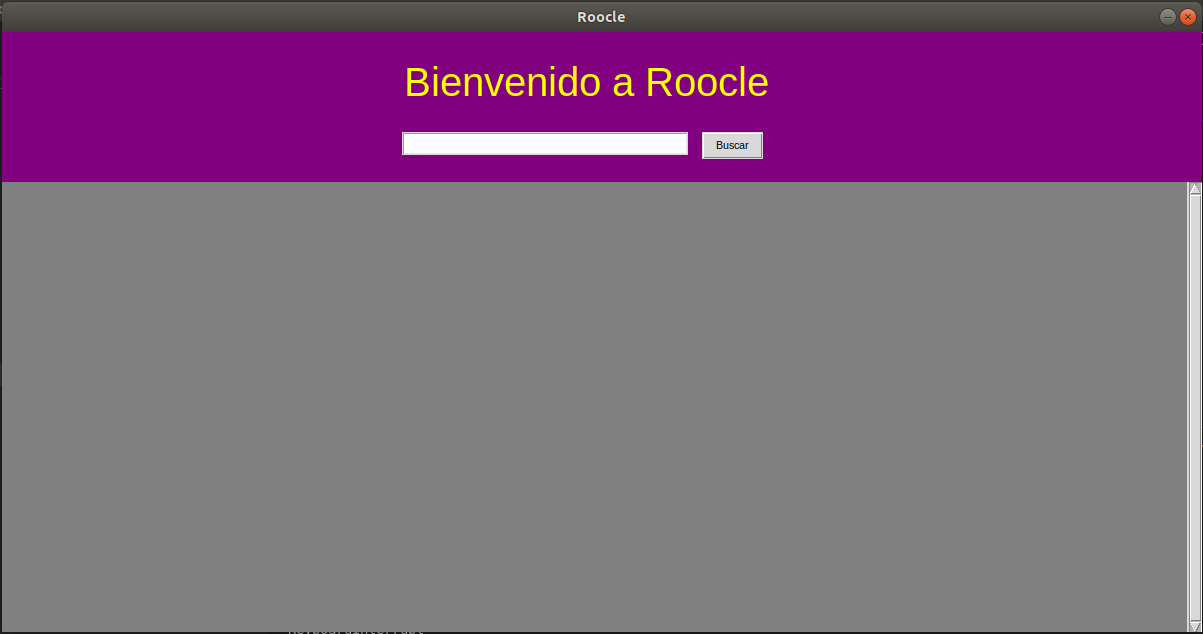
\includegraphics[width =12.0cm]{inicio.png}
			\caption[Fig1]{Inicio de la aplicaci\'on}		
		\end{center}
	\end{figure}
	
	Para realizar una consulta la escribimos en la barra que aparece debajo del cartel de bienvenida y presionamos el bot\'on ``Buscar''. Al hacer esto la aplicaci\'on mostrar\'a los 10 documentos m\'as similares a la consulta realizada. Por ejemplo veamos, en la Fig 2, que se obtiene al realizar la primera consulta de la colecci\'on \textbf{Cranfield}.
	
	\begin{figure}[h]
		\begin{center}
			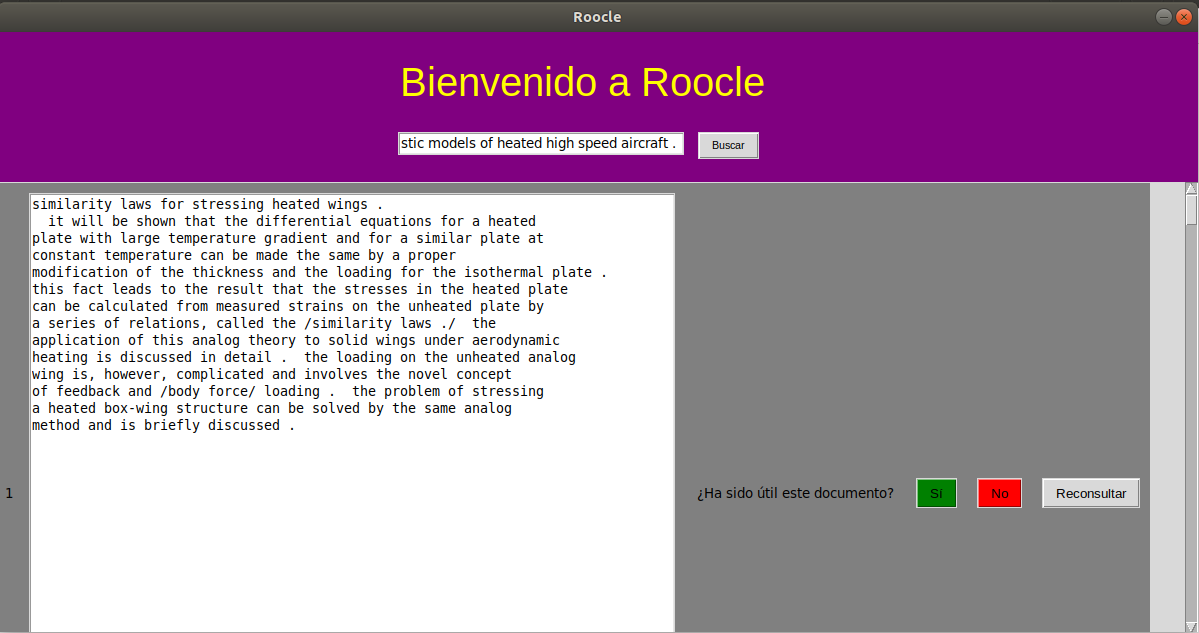
\includegraphics[width =12.0cm]{consulta.png}	
			\caption[Fig2]{Ejemplo de consulta (Cranfield)}	
		\end{center}
	\end{figure}
	
	En la Fig. 2 vemos el documento m\'as similar a la consulta, para ver el resto de documentos utilizamos la \textit{scrollbar} situada a la derecha.
	
	Ahora obs\'ervese que a la derecha del documento aparece la pregunta de si >Ha sido \'util el documento? Y a la derecha de esta dos botones: ``S\'i'' y ``No''. El usuario al presionar uno de estos botones indica si el documento es relevante o no. Esta informaci\'on luego se utiliza para el proceso de retroalimentaci\'on.
	
	Por \'ultimo se observa tambi\'en el bot\'on ``Reconsultar'' que este solo aparece una vez (a la derecha del documento m\'as similar) y al presionar en \'el se indica que se rehaga la consulta con la informaci\'on de relevancia e irrelevancia de los documentos. O sea, se vuelve a calcular la similitud utilizando como vector consulta el devuelto por el Algoritmo de Rocchio.
	
	En la Fig. 3 se presenta un segundo ejemplo utilizando la colecci\'on \textbf{Medline}, realizando la primera consulta de esta colecci\'on.
	
\begin{figure}[h]
	\begin{center}
		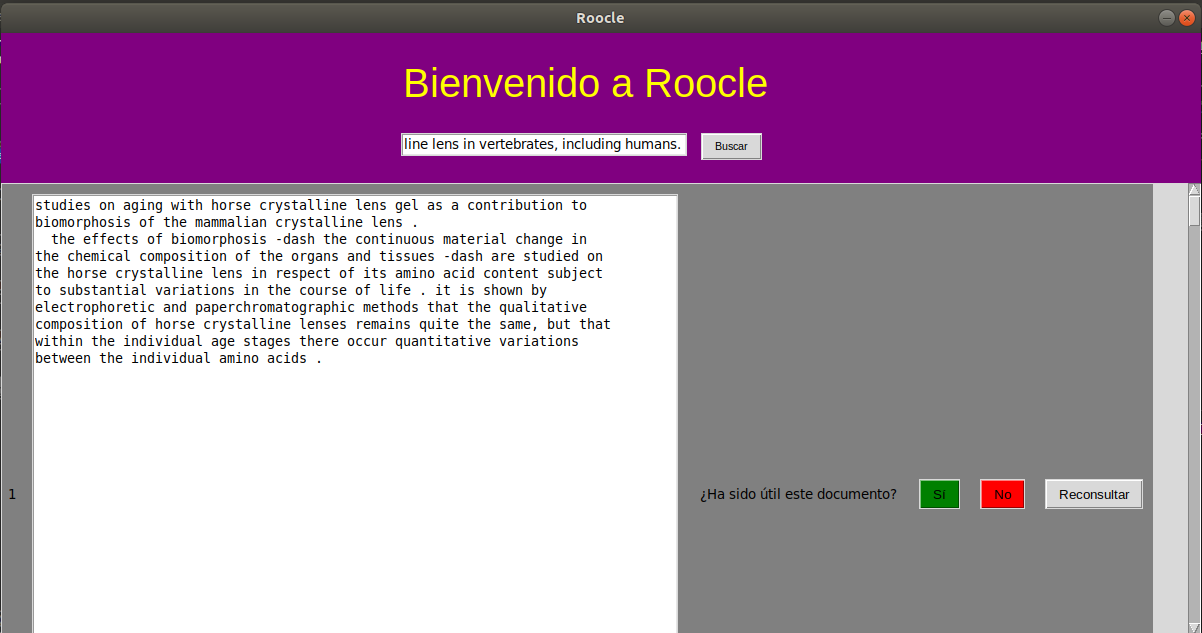
\includegraphics[width =12.0cm]{consulta_2.png}	
		\caption[Fig3]{Ejemplo de consulta (Medline)}	
	\end{center}
\end{figure}

	\section{An\'alisis de los resultados del sistema}
	
	\subsection{Explicaci\'on de las Medidas}
	Para el an\'alisis de los resultados del sistema se implementaron un conjunto de medidas que caracterizan el sistema de acuerdo a los documentos que recupera y los que no. En esto se destacan siete conjuntos fundamentales de documentos:
	\begin{itemize}
	\item Conjunto de documentos relevantes (REL)
	\item Conjunto de documentos irrelevantes (I)
	\item Conjunto de documentos recuperados (REC)
	\item Conjunto de documentos recuperados relevantes (RR)
	\item Conjunto de documentos recuperados no relevantes (RI)
	\item Conjunto de documentos no recuperados relevantes (NR)
	\item Conjunto de documentos no recuperados irrelevantes (NN)
	\end{itemize}
	
	Por la propia definic\'on de estos conocemos que se cumple la relaci\'on de la Fig 4.
	
	\begin{figure}[h]
		\begin{center}
			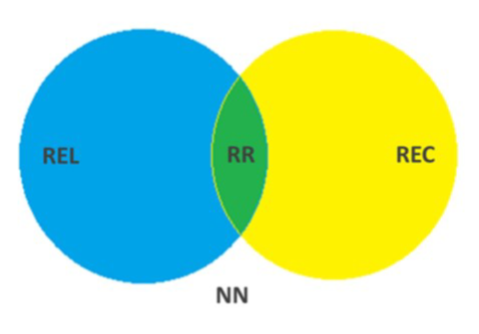
\includegraphics[width =8.0cm]{Diagrama.png}
			\caption[Fig 4]{Relaci\'on entre los conjuntos de documentos}		
		\end{center}
	\end{figure}
	
	A continuaci\'on se enuncian las medidas implementadas y se explica la idea utilizada.
	
\subsubsection{Precisi\'on }

	Esta medida caracteriza la respuesta a la consulta seg\'un los documentos relevantes que se recuperaron
	\begin{align*}
	P&=\dfrac{|RR|}{|REC|}
	\end{align*}
	
	Esta medida tiende a decrecer cuando aumentan los documentos recuperados. Para calcularla, una vez hallados los documentos relevantes para la consulta, utilizando la informaci\'on de apoyo de la colecci\'on, se analiz\'o cu\'ales se hab\'ian recuperado y de estos los que estaban entre los relevantes y se aplic\'o la f\'ormula. Esto  se hizo para cada consulta de la colecci\'on y los resultados obtenidos se promediaron. 

\subsubsection{Recobrado}

Esta medida es fundamental en los procesos de recuperaci\'on de informaci\'on.
	\begin{align*}
	R&=\dfrac{|RR|}{|REL|}
	\end{align*}
	Para calcularla, una vez obtenidos los documentos relevantes para la consulta se analiz\'o de ellos cu\'antos se recuperaron, para aplicar la f\'ormula. De esta forma se procedi\'o en cada consulta de la colecci\'on y se promediaron los resultados.
\subsubsection{Medida F}

Esta medida permite enfatizar la precisi\'on sobre el recobrado o viceversa:
	\begin{align*}
	F&=\dfrac{(1+ \beta^{2})PR}{\beta^{2} P + R}
	\end{align*}
	
$ \beta < 1 $ el recobrado tiene mayor peso

$ \beta = 1 $ la precisi\'on y el recobrado tienen igual peso

$ \beta > 1 $ la precisi\'on tiene mayor peso

Para hallar esta medida se utiliz\'o el c\'alculo de las dos anteriores  y se promedi\'o para cada consulta de la colecci\'on.
\subsubsection{Medida F1}
Esta medida armoniza precisi\'on y recobrado teniendo en cuenta ambos.
	\begin{align*}
	F1&=\dfrac{2PR}{P + R}
	\end{align*}
	F1 tendr\'a un valor alto si la precisi\'on y el recobrado son altos, luego puede interpretarse como un esfuerzo por hallar el mejor compromiso entre ambos. Para el c\'alculo de esta se tom\'o de apoyo los c\'alculos de precisi\'on y recobrado anteriormente explicados y se promedi\'o para cada consulta de la colecci\'on.
	
\subsubsection{R-Precisi\'on}

Esta medida es el ranking de documentos relevantes a una consulta para la cuál existen R documentos relevantes.
	\begin{align*}
	P_{R}&=\dfrac{|RR|_{R}}{R}
	\end{align*}
	
	Para esta medida se seleccionaron los R primeros documentos recuperados y de estos se analiz\'o cu\'ales eran relevantes para la consulta. Esto se hizo para cada consulta de la colecci\'on y se promediaron los resultados obtenidos.

\subsubsection{Proporci\'on de fallo}
Tiene en cuenta la cantidad de documentos irrelevantes 
	\begin{align*}
	Fallout&=\dfrac{|RI|}{|I|}
	\end{align*}
	Para su c\'alculo, se tomaron los documentos relevantes para la consulta y los documentos recuperados. Con la diferencia entre el conjunto de todos los documentos y el conjunto de todos los documentos relevantes para determinada consulta se obtuvieron los documentos irrelevantes para la misma. Luego se compararon de estos cu\'ales se recuperaron y se aplic\'o la f\'ormula. Se procedi\'o de la misma forma para cada consulta y se promediaron los resultados.
	
\subsection{An\'alisis de los Resultados}
Para cada consulta, utilizando la colecci\'on \textbf{Cranfield} (que cuenta con 1400 documentos y 225 consultas) y retornando los documentos cuya similitud con la consulta es mayor o igual a 0.1, se obtuvieron los siguientes resultados:

\begin{itemize}
\item Precisi\'on promedio:  0.15463199286061183
\item Recobrado promedio:  0.6024723852836802
\item R-precisi\'on5 promedio:  0.409777777777778
\item Medida\_F promedio  $ \beta=0 $:  0.15463199286061183 
\item Medida\_F promedio  $ \beta=2 $:  0.33108870640070265
\item Medida\_F1 promedio: 0.22145562556179862
\item Proporci\'on de fallo  promedio:  0.10862096867414041
\item R-fallout5 promedio:  0.012918518518518506
\end{itemize}

Se observa una baja precisi\'on promedio, sin embargo la R-precisi\'on5 promedio es mucho m\'as alta. El recobrado promedio lo podemos catalogar de aceptable.

Utilizando un umbral de similitud de 0.2 se obtienen los siguientes resultados:

\begin{itemize}
\item Precisi\'on promedio:  0.43399651574757653
\item Recobrado promedio:   0.34757621509916814
\item R-precisi\'on5 promedio:  0.3591111111111116
\item Medida\_F promedio  $ \beta=0 $:  0.43399651574757653 
\item Medida\_F promedio  $ \beta=2 $:  0.32329056742389967
\item Medida\_F1 promedio:    0.32206114272154335
\item Proporci\'on de fallo promedio: 0.021765179813960357
\item R-fallout5 promedio: 0.007901234567901236 
\end{itemize}

Se aprecia como la precisi\'on promedio aument\'o en gran medida pero sin embargo el recobrado disminuy\'o bastante. Incluso la R-precisi\'on5 disminuye debido a que para muchas consultas se devuelven menos de 5 documentos.

Por \'ultimo si se fija el umbral de similitud en 0.15 se obtienen los siguientes resultados:

\begin{itemize}
	\item Precisi\'on promedio:   0.28814475479798424
	\item Recobrado promedio:  0.45801026483780116
	\item R-precisi\'on5 promedio:  0.402666666666667
	\item Medida\_F promedio  $ \beta=0 $:   0.28814475479798424
	\item Medida\_F promedio  $ \beta=2 $:  0.3532712231591747
	\item Medida\_F1 promedio:     0.29718448265513353
	\item Proporci\'on de fallo promedio: 0.044796004410715566
	\item R-fallout5 promedio:  0.011377777777777777 
\end{itemize}

Para este umbral de similitud se aprecia una compensaci\'on en cuanto a los valores de precisi\'on y recobrado pero a\'un as\'i los valores obtenidos no son los mejores.

Si nos fijamos en la Medida\_F1 se puede apreciar que el mejor resultado se obtiene cuando el umbral de similitud es 0.2.

Pasemos ahora analizar el sistema con la colecci\'on \textbf{Medline} (que cuenta con 1033 documentos y 30 consultas) y con umbral de similitud 0.1: 

\begin{itemize}
	\item Precisi\'on promedio:  0.6101614388092593
	\item Recobrado promedio:  0.4688505534796139
	\item R-precisi\'on5 promedio: 0.6933333333333335
	\item Medida\_F promedio  $ \beta=0 $:    0.6101614388092593
	\item Medida\_F promedio  $ \beta=2 $:  0.4608114878487888
	\item Medida\_F1 promedio:    0.47236203447374764
	\item Proporci\'on de fallo promedio: 0.16790582403965298
	\item R-fallout5 promedio:  0.04444444444444446
\end{itemize}

Como se puede apreciar con este umbral de similitud la precisi\'on promedio es aceptable y el recobrado se acerca al 50$\%$. La R-precisi\'on5 promedio es bastante buena.

Utilizando ahora un umbral de similitud de 0.05 se obtienen los siguientes resultados:

\begin{itemize}
	\item Precisi\'on promedio:  0.3530530523152345
	\item Recobrado promedio:  0.7007911295917294
	\item R-precisi\'on5 promedio:  0.7200000000000002
	\item Medida\_F promedio  $ \beta=0 $:    0.3530530523152345
	\item Medida\_F promedio  $ \beta=2 $:   0.5464053607927845
	\item Medida\_F1 promedio:    0.4373855559506214
	\item Proporci\'on de fallo promedio: 0.6087398373983741
	\item R-fallout5 promedio:  0.04666666666666668
\end{itemize}

Se aprecia como la precisi\'on promedio disminuy\'o bastante, contrario al recobrado que aument\'o en gran medida su valor. La R-precisi\'on5 aument\'a un poco su valor debido a que al bajar el umbral de similitud, consultas para las que se recuperaban menos de 5 documentos, ahora se devuelven 5 o m\'as. Al bajar tambi\'en el umbral de similitud tambi\'en aument\'o en gran medida la proporci\'on de fallo promedio, aunque el R-fallout5 no vari\'o mucho su valor.

Por \'ultimo veamos ahora los resultados obtenidos utilizando 0.08 como umbral de similitud:

\begin{itemize}
	\item Precisi\'on promedio:  0.5377846857131453
	\item Recobrado promedio:  0.5580216992563317
	\item R-precisi\'on5 promedio:  0.7200000000000002
	\item Medida\_F promedio  $ \beta=0 $:     0.5377846857131453
	\item Medida\_F promedio  $ \beta=2 $:   0.5205735784074199
	\item Medida\_F1 promedio:    0.4979325593246483
	\item Proporción de fallo promedio: 0.25763239875389343
	\item R-fallout5 promedio:  0.04555555555555557
\end{itemize}

Se aprecia una la existencia de una compensaci\'on entre la precisi\'on y el recobrado. La R-precisi\'on5 es bastante buena.

Comparando las Medidas\_F1 con los diferentes valores de umbrales de similitud el mejor resultado se obtiene utilizando 0.08.

El c\'odigo correspondiente a estos an\'alisis se encuentra en el archivo ``system\_evaluation.py'', al ejecutarlo es necesario especificar, en la l\'inea 16, la direcci\'on del archivo que contiene las relaciones de relevancia de la \'ultima colecci\'on procesada. Los valores de umbral de similitud se fijan en la l\'inea 14.



\section{An\'alisis de la aplicaci\'on}
\subsection{Ventajas}
\begin{itemize}
\item Utiliza el modelo vectorial por lo que los documentos se ordenan de acuerdo al grado de similitud con la consulta, puedi\'endose recuperar documentos que se aproximen a los requerimientos de la consulta.
\item Presenta una interfaz gr\'afica, de forma que sea m\'as accesible y c\'omoda para los usuarios.
\item Utiliza la retroalimentaci\'on para mejorar las respuestas a las consultas de acuerdo al criterio del usuario.
\item Tiene una baja proporci\'on de fallo.
\end{itemize}
\subsection{Desventajas}
\begin{itemize}
\item Utiliza un modelo vectorial por lo que asume que todos los t\'erminos indexados son mutuamente independientes.
\item No se integr\'o con algoritmos de Crawling.
\item No se usa bases de conocimiento como tesauros u ontolog\'ias.
\item Puede ser dif\'icil lograr una buena compensaci\'on entre la precisi\'on y el recobrado.
\end{itemize}

\section{Conclusiones}
En funci\'on de lo planteado en las secciones anteriores se arriban a las siguientes conclusiones:
	
	\begin{itemize}
	\item Se dise\~{n}\'o un Sistema de Recuperaci\'on de Informaci\'on para una colecci\'on de documentos dada.
	\item Se realiz\'o una interfaz gr\'afica para brindar comodidad al usuario.
	\item Se implement\'o la retroalimentaci\'on para el sistema de forma que mediante la ayuda del usuario se perfeccione su funcionamiento.
	\item Se analizaron los resultados obtenidos por el sistema con vistas a evaluar el funcionamiento del mismo.
	\end{itemize}
	
	\section{Recomendaciones}
	En virtud del trabajo realizado y las posibilidades del mismo se recomienda:
	\begin{itemize}
	\item Ampliar el proyecto mediante la integraci\'on con algoritmos de Crawling y a\~{n}adiendo bases de conocimiento como ontolog\'ias o tesauros.
	\item Utilizar t\'ecnicas m\'as avanzadas de recuperaci\'on de informaci\'on para obtener mejores resultados, sobre todo en la precisi\'on y el recobrado.
	\item Utilizar t\'ecnicas m\'as avanzdas para el preprocesamiento de de documentos y  consultas lo cual conllevar\'ia a la obtenci\'on de mejores resultados.
	\end{itemize}
	
	\begin{thebibliography}{1}
		\item Conferencias de Sistemas de Recuperaci\'on de Informaci\'on. Curso 2021-2022.
		\item \href{https://m.youtube.com/channel/UCfzlCWGWYyIQ0aLC5w48gBQ}{Canal de yotube: sentdex}
		\item \href{https://docs.python.org/3/library/heapq.html}{Documentaci\'on de python sobre heap}
	\end{thebibliography}

\end{document}